\documentclass[11pt,a4paper]{article}

\usepackage[margin=1in, paperwidth=8.3in, paperheight=11.7in]{geometry}
\usepackage{amsmath,amsfonts,fancyhdr,bbm,graphicx,tikz}
\usepackage{float,hyperref}
\usetikzlibrary{automata,positioning}
\graphicspath{ {img/} }
\usepackage[section,nohyphen]{DomH}
\headertitle{Applied Data Science - Notes}

\begin{document}

\title{Applied Data Science - Notes}
\author{Dom Hutchinson}
\date{\today}
\maketitle

\tableofcontents\newpage

\section{Introduction}\label{sec_introduction}

  \begin{remark}{Types of Data}
    Data comes in many forms including, but not limited to, the following
    \begin{itemize}
      \item Dense \& Sparse data.
      \item Structured/Relational Data.
      \item Numerical; Categorical; Ordinal; or Boolean.
      \item Test (Emails, Tweets, Articles).
      \item Records (User-Level Data, Timestamped Event Data, Log Files).
      \item Geo-Based Location Data.
      \item Data-Time Data.
      \item Network Data.
      \item Sensor Data.
      \item Images and Video.
      \item Audio and Music.
    \end{itemize}
  \end{remark}

  \begin{remark}{Big \& Small Data}
    Whether a dataset is big or small depends on the computational-resources available, and thus will vary over time. Here are some ways to evaluate this
    \begin{center}
      \begin{tabular}{l|p{6cm}|p{6cm}}
        &\textbf{Big Data}&\textbf{Small Data}\\\hline
        \textit{Data Condition}&Always unstructured, not read for analysis, many relational database tables that need to be merged.&Ready for analysis, flat file, no need to merge tables.\\\hline
        \textit{Location}&Cloud, offshore, SQL server etc.&Database, local PC.\\\hline
        \textit{Data Size}&Over 50k variables, over 50k individuals, random samples, unstructured&File that is in a spreadsheet, that can be viewed on a few sheets of paper.\\\hline
        \textit{Data Purpose}&No intended purpose.&Intended purpose for data collection.
      \end{tabular}
    \end{center}
  \end{remark}

  \begin{remark}{What is Data Science?}
    Data-Driven Science. An interdisciplinary field about scientific processes and systems to extract knowledge or insights from data in various forms.
    \par Data science incorporates fields from: Mathematics, Computer Science; \&, Domain Expertise.
  \end{remark}

  \begin{remark}{Motivating Applications}
    Data science is motivated by its applications. Here are some examples of such applications
    \begin{itemize}
      \item \textit{Amazon} use recommender systems to suggest products to customers.
      \item \textit{Energy Companies} use data science to try and predict future usage of customers, so that resources can be applied efficiently.
      \item \textit{Agriculture} use sensors in fields to collect data in order to monitor crops and predict weather.
      \item \textit{Healthcare} use sensors in homes to monitor the health of people over long periods of time (especially when the person cannot go to the hospital).
    \end{itemize}
  \end{remark}

  \begin{figure}[H]
    \centering
    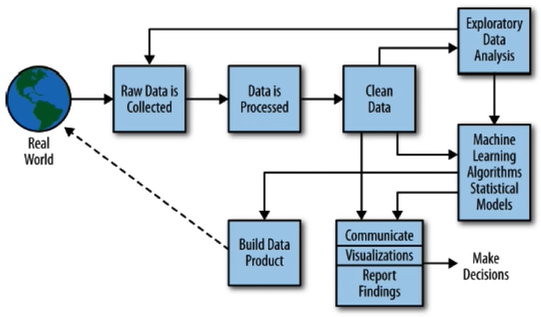
\includegraphics[width=.7\textwidth]{DataSciencePipeline.PNG}
    \caption{The pipeline for approaching problems in data science.}
    \label{fig_DataSciencePipeline}
  \end{figure}

  \begin{proposition}{Data Science Pipeline}
    See \texttt{Figure \ref{fig_DataSciencePipeline}} for a pipeline for approaching data science problems.
  \end{proposition}

\section{Data Ingress \& Pre-Processing}\label{sec_data_ingress}

\subsection{Data Structures}

  \begin{proposition}{Native Python Data Structures}
    Here are some data structures which are native to python and are popular in data science
    \begin{itemize}
      \item \texttt{list} - List of elements of varying types.
      \item \texttt{set} - List of unique elements of varying types.
      \item \texttt{dict} - Key-Value pairings.
    \end{itemize}
  \end{proposition}

  \begin{proposition}{Non-Native Python Data Structures}
    Here are some data structures which are \underline{not} native to python but are popular in data science.
    \begin{itemize}
      \item \texttt{np.array}.
      \item \texttt{pandas.DataFrame}.
    \end{itemize}
  \end{proposition}

\subsection{Data Formats}

  \begin{definition}{Object Persistence}
    \textit{Object Persistence} is the process of ensuring that the objects which are created are kept through multiple sessions. This comes in two stages
    \begin{enumerate}
      \item \textit{Serialisation} - Translating data structures or objects from memory into a format which can be stored.
      \item \textit{Deserialisation} - The inverse. Translating data structures which have been stored, into memory.
    \end{enumerate}
  \end{definition}

  \begin{remark}{Bespoke Serialisation \& Deserialisation}
    Bespoke serialisation and deserialisation methods can be crafted manually. (e.g. Instantiating an output file; Writing each element of a list to a different line in the file; Closing the file.)
    \par However, there are limitations to bespoke methods:
    \begin{itemize}
      \item Methods are specific to each use case (not standardised).
      \item Methods may not be robust.
      \item Methods require testing against many test cases.
      \item Object metadata is not encoded.
    \end{itemize}
    These limitations are rarely a problem in very controlled environments.
  \end{remark}

  \begin{definition}{Comma-Separated Values (CSV)}
    \textit{Comma-Separated Values} (CSV) files are well suited to tabular data (inc. matrices). Each line of a \textit{CSV File} stores one row of the table, and each element in a row is separated by a comma.
    \par \textit{CSV Files} are generally very readable, as well as time- and space-efficient for tabular data.
  \end{definition}

  \begin{remark}{Using CSV Files}
    As \textit{CSV Files} are very popular, there are many library methods which can interact with them. Including reading \& writing to and from memory (e.g. \texttt{pandas.read\_csv}).
  \end{remark}

  \begin{definition}{JavaScript Object Notation (JSON)}
    \textit{JavaScript Object Notation}\footnote{JSON is not just compatible with JavaScript and is common for many languages \& APIs} (JSON) is a standardised syntax for storing \& exchanging data, used for serialisation. JSON uses text files which are human-readable and \texttt{dict}-like (i.e. have value-key pairs). JSON is designed to be simple so is a very robust language \& suits many purposes.\footnote{\url{https://jsonlint.com/} is a useful site for JSON validation.}
    \par Limitations of JSON are that a specific conversion process may be required to convert a JSON file into objects in memory, and JSON files can become large due to key repetition.
  \end{definition}

  \begin{definition}{Hierarchical Data Format (HDF5)}
    \textit{Hierarchical Data Format} (HDF5) is a standardised format for serialisation. HDF5 is a binary format and tries to mimic  file system-like access. HDF5 files have the following three components
    \begin{enumerate}
      \item \textit{Datasets} - Array-like collections of data. Thousands of datasets can be stored in a single file, and can be categorised and tagged however you want.
      \item \textit{Groups} - Folder-like structures which groups datasets \& other groups.
      \item \textit{Metadata} - Information which pertains to all the datasets. (e.g. author, edit data \& version).
    \end{enumerate}
    \par HDF5 files are ideal for large numerical data sets, and can easily be manipulated by \texttt{numpy}. HDF5 files support a variety of transparent storage features (inc. compression, error-detection and chunked I/O), which \texttt{numpy.array} do not.\footnote{\url{http://docs.h5py.org/en/latest/quick.html} provides a quick-start guide to using HDF5 files in python.}
  \end{definition}

  \begin{proposition}{HDF5 files vs Traditional File Systems}
    There are a few key differences between \textit{HDF5 Files} and \textit{Traditional File Systems}.
    \begin{enumerate}
      \item \textit{HDF5 Files} are portable, as the entire structure is contained in the file independent of the underlying file system.\footnote{However, it does depend on the HDF5 library.}
      \item Datasets in \textit{HDF5 Files} are all homogeneous hyper-rectangular numerical arrays, whereas files in traditional file system can be anything.
      \item Metadata can be added to groups in \textit{HDF5 Files}. This is not possible in traditional file systems.
    \end{enumerate}
  \end{proposition}

  \begin{remark}{Other Standardised Serialisation Method}
    XML, \textit{Protocol Buffers} \& YAML are other popular standardised serialisation methods.
  \end{remark}

\subsection{Web-Scraping \& APIs}

  \begin{remark}{Terms of Use}
    \textit{Web Scraping} should be done within the website's terms of use.
  \end{remark}

  \begin{definition}{Web Scraping}
    \textit{Web Scraping} is the practice of collecting data from websites. This can take many forms, but typically involves taking a raw webpage and parsing the desired data.
  \end{definition}

  \begin{proposition}{Approaching Web Scraping}
    To perform \textit{Web Scraping} successfully, you need a good idea of how a webpage is structure. Typically webpages are based around a \texttt{html} file, which are well structured\footnote{Webpages are often interpreted to have a tree structure, with each tag being a node}. Identifying combinations of tags, classes \& ids in the \texttt{html}  file can help locate the desired data.
    \par It is harder, sometimes impossible, to navigate poorly designed websites as they are less structured and inconsistent.
  \end{proposition}

  \begin{remark}{Tools for Web Scraping}
    \textit{Web Scraping} technologies need to be tolerant to several artefacts of real-world data (known as \textit{"wrangling"}) as-well-as errors in the website.
    \par Some popular tools for \textit{Web Scraping} are
    \begin{itemize}
      \item \texttt{BeautifulSoup} - A python library for parsing \texttt{XML} \& \texttt{HTML}.
      \item \texttt{scrapy} - A python library. Generally faster than \texttt{BeautifulSoup}.
      \item \texttt{Selenium} - A web-browser plugin, generally used to test web services.
    \end{itemize}
  \end{remark}

  \begin{definition}{Web APIs}
    \textit{Web APIs} greatly simplify \textit{Web Scraping} by provide a portal for explicit data acquisition, and are generally less prone to the issues which arise when \textit{Web Scraping}.\footnote{See \url{https://github.com/public-apis/public-apis} for a categorised list of public APIs.}
    \begin{itemize}
      \item The code running \textit{Web APIs} is optimised for data requesting \& retrieval. It does not waste time on visualisation or aesthetics. This means the bandwidth required for an \textit{API} request is much lower than for a similiar \textit{Web Scraping} process (As images etc. do not need to be loaded).
      \item \textit{Web API} querying is robust, reliable, well maintained and documented with a static schema (\texttt{HTML}-based \textit{Web Scraping} is not).
      \item \textit{Web APIs} use standardised \textit{Serialisation Tools} (e.g. JSON).
      \item \textit{Web APIs} have already extracted and organised the desired data, however this does mean the user can only access what the operator will allow. This is much better than \texttt{HTML}-based \textit{Web Scraping} where you rely upon fickle naming conventions of tags.
    \end{itemize}
  \end{definition}

  \begin{definition}{RESTful APIs}
    \textit{Representational State Transfer APIs} (REST/RESTful) are a popular form of \textit{Web API} and generally require an \textit{API Key} to access data.
    \par Request to \textit{RESTful APIs} generally involves constructing a URL which contains your keys and the parameters of your query.
  \end{definition}

  \begin{remark}{Regular Expression (RegEx)}
    \textit{Regular Expression} (ReGex) queries are useful for extracting data, either while web scraping or from API requests.\footnote{\url{http://pythex.org/} is a website which can perform \textit{RegEx}.} Python has the \texttt{re} library for \textit{RegEx} queries, two popular methods from this library are
    \begin{enumerate}
      \item \texttt{re.match} - Attempts to match a \textit{RegEx} pattern to the whole string.
      \item \texttt{re.search} - Searches for the \underline{first} occurrence of a \textit{RegEx} pattern in a string.
    \end{enumerate}
  \end{remark}

\section{Privacy}\label{sec_privacy}

\subsection{IRL Examples}

  \begin{remark}{AOL Data Incident, 2006}
    In 2006, \textit{AOL Research} released to the public, for the purpose of research, a text file containing 20mn search terms from over 650k users, over a 3-month period.
    \par The users were anonymised in the in the data, but personally identifiable information was present in many of the search terms.
    \par \textit{AOL Research} retracted the document shortly after publishing.
  \end{remark}

  \begin{remark}{Netflix Prize, 2007}
    In 2007, \textit{Netflix} ran a competition where \$1mn was offered to anyone who was able to produce a system which outperformed their existing recommender system by at least 10\%.
    \par The training data offered by \textit{Netflix} contained <user,movie,date,grade> and customer ids were anonymised.
    \par It was later found that some users had their \textit{Netflix} and \textit{IMDb} accounts linked (so reviews were posted on both). This meant the training data could be partially de-anonymised. This led to lawsuits and \textit{Netflix} cancelling future competitions.
  \end{remark}

  \begin{remark}{Pay Attention}
    The moral of these examples is that you have to be really careful and diligent when anonymising data as there may be non-obvious ways for people to de-anonymise it. (Often through little fault of your own).
  \end{remark}

\subsection{Security \& Statistical Database}

  \begin{definition}{Statistical Database}
    A \textit{Statistical Database} is a database for statistics. They can come in several forms
    \begin{itemize}
      \item \textit{Tabular Data} - Tables with counts or magnitudes.
      \item \textit{Queryable Databases} - On-line databases which accept statistical queries (e.g. min, max, sum etc.)
      \item \textit{Microdata} - Files where each record contains information about an individual.
    \end{itemize}
  \end{definition}

  \begin{remark}{Privacy Trade-Off}
    \textit{Statistical Databases} have to trade-off privacy and functionality. Generally, more privacy means less functionality.
  \end{remark}

  \begin{definition}{Identifiers}
    \textit{Identifiers} are attributes that unambiguously identify someone (e.g. passport number, NI number, name etc.)
  \end{definition}

  \begin{definition}{Quasi-Identifiers}
    \textit{Quasi-Identifiers} are attributes which identify someone, but there is some ambiguity. Often, having multiple \textit{Quasi-Identifiers} are enough to confidently identify someone. (e.g. address, age, gender).
  \end{definition}

  \begin{definition}{Confidential Attributes}
    \textit{Confidential Attributes} are attributes which contain sensitive information about an individual (e.g. salary, religion, medical conditions etc.)
  \end{definition}

  \begin{definition}{Non-Confidential Attributes}
    \textit{Non-Confidential Attributes} are attributes which do \underline{not} contain sensitive information about an individual.
  \end{definition}

  \begin{remark}{Anonymisation, Identifiers \& Quasi-Identifiers}
    When anonymising a data set:
    \begin{itemize}
      \item \textit{Identifiers} need to be suppressed from the data sets (i.e. removed).
      \item \textit{Quasi-Identifiers} hold disclosure risk as they can often not be suppress due their high analytical value, but can often be linked with other non-anonymised datasets to de-anonymise your dataset.
    \end{itemize}
  \end{remark}

  \begin{definition}{Attribute Disclosure}
    \textit{Attribute Disclousure} is when the value of a confidential attribute is made available, and in doing so the individual is easier to identifier (compared to the value not being disclosed).
  \end{definition}

  \begin{definition}{Identity Disclosure}
    \textit{Identity Disclosure} is when an entire record in an anonymised data set can be linked with that individual's identity.
  \end{definition}

  \begin{definition}{Membership Disclosure}
    \textit{Membership Disclosure} is whether or not data about an individual is contained in a dataset.
  \end{definition}

  \begin{definition}{External Attack on a Table}
    An \textit{External Attack} on a table occurs when another dataset is released which contains data which comprises more table, or can be combined with your table to comprise others.
  \end{definition}

  \begin{definition}{Internal Attack on a Table}
    An \textit{Internal Attack} on a table occurs when those within the table (i.e. with access to it and know which data represents them) are able to deduce which data belongs to other people by a process of elimination.
    \par Only really possible when the table has few respondents.
  \end{definition}

  \begin{definition}{Dominance Attack on a Table}
    An \textit{Internal Attack} on a table occurs a (or a few) respondents dominate the contribution in a particular cell of a magnitude table, these \textit{Dominant Respondents} are then able to upper-bound the contributions from the rest due it being easier to differentiate other users from them.
  \end{definition}

  \begin{proposition}{Combatting Table Attacks}
    There are two main approaches to combatting \textit{Table Attacks}
    \begin{enumerate}
      \item \textit{Non-Perturbative} techniques which do \underline{not} modify the values in the cells, but they may suppress or recode them (e.g. cell suppression, recoding of categorical attributes).
      \item \textit{Perturbative} techniques do modify the values in the cells (e.g. controlled rounding).
    \end{enumerate}
  \end{proposition}

  \begin{proposition}{Combatting Database Attacks}
    There are three main approaches to combatting attacks on databases, all focused around adjusting/controlling queries
    \begin{enumerate}
      \item \textit{Query Input Perturbation} - Perturbation is applied to records on which queries are computed.
      \item \textit{Query Output Perturbation} - Perturbation is applied to the results of a query.
      \item \textit{Query Restriction} - The database refuses certain queries.
      \item \textit{Camoflage} - Returns answers which have been made non-exact in some deterministic fashion.
    \end{enumerate}
  \end{proposition}

  \begin{remark}{Differential Attack\footnote{Not proper name.}}
    Suppose you know that someone is going to be changing doctors soon (and thus will be removed from the doctors database), if you copied the database before and after this person moves you could likely deduce details about the individual by comparing the two versions.
    \par How do we prevent this?
  \end{remark}

  \begin{definition}{Differential Privacy}
    Consider a learner implements a summary statistic $A$ (e.g. sum of all elements); an adversary proposes two datasets $S$ and $S'$ which differ by only one row; and a test set $Q$. The learner wants the summary statistic to have the same value if only one row has changed.
    \par Summary statistic $A$ is \textit{$\varepsilon$-Differentially Private} iff
    \[ \left|\ln\left(\frac{\prob(A(S)\in Q)}{\prob(A(S')\in Q)}\right)\right|\leq\varepsilon \]
    Note that \textit{Differential Privacy} is a condition on the release mechanism of the data $A$, not on the data $S,S'$ itself.
  \end{definition}

  \begin{remark}{Differential Privacy in Practice}
    In practice we avoid differential privacy issues by adding noise to our responses (either to all responses, or incorrectly responding to some queries).
  \end{remark}

\subsection{$k$-Anonymity}

  \begin{definition}{$k$-Anonymity}
    A dataset satisfies \textit{$k$-Anonymity} if each combination of values of \textit{Quasi-Identifier Attributes} in the table are shared by at least $k$ records.
    \par Measuring \textit{$k$-Anonymity} requires a brute force approach which compares every pair of records in the table.
  \end{definition}

  \begin{proposition}{Achieving $k$-Anonymity}
    There are two main approaches to achieving \textit{$k$-Anonymity}:
    \begin{itemize}
      \item \textit{Suppression} - Replace the values of attributes with an asterisk.
      \item \textit{Generalisation} - Values of attributes are replaced with a broader category. (e.g. age-ranges rather than exact age)
    \end{itemize}
  \end{proposition}

  \begin{proposition}{$k$-Anonymity Attacks}
    \textit{$k$-Anonymity} does not protect against attribute disclosure attacks in general if the values of \textit{Confidential Attributes} are very similar in the group of $k$ records who share \textit{Quasi-Identifier} values.
    \par Here are two specific attacks that can happen
    \begin{itemize}
      \item \textit{Homogeneity Attack} - If all records in the set of $k$ identical records have the same \textit{Sensitive Value}, then the value can likely be predicted (and would comprise all $k$).
      \item \textit{Background Knowledge Attack} - If associations exist between one or more \textit{Quasi-Identifier Attributes} and a \textit{Sensitive Attribute} then the set of possible values of the \textit{Sensitive Attribute} is reduced.
    \end{itemize}
  \end{proposition}

  \begin{definition}{$l$-Diversity}
    \textit{$l$-Diversity} is an extension of \textit{$k$-Anonymity}.
    \par \textit{$l$-Diversity} requires that the values of all \textit{Confidential Attributes} within any group of $k$-anonymous records contain at least $l$ clearly distinct values.
  \end{definition}

  \begin{proposition}{Limitations of $l$-Diversity}
    Here are two limitations of \textit{$l$-Diversity}
    \begin{itemize}
      \item Not every value shows equal sensitivity. (A rare positive indicator for a disease may provide more information than a common negative indicator).
      \item It ensures diversity of sensitive values in each group, but it does not recognise that values may be semantically similar.
    \end{itemize}
  \end{proposition}

  \begin{definition}{$t$-Closeness}
    \textit{$t$-Closeness} requires that the distribution of the confidential attribute within a group of $k$ records is similar to the distribution of the confidential attribute in the entire data set (at most distance $t$ between the two distributions).
  \end{definition}

  \begin{remark}{Tools for Anonymisation}
    Here are three popular tools for anonymisation
    \begin{enumerate}
      \item \textit{ARX} - Applies $k$-anonymity, $l$-diversity and $t$-clossness in Java.
      \item \textit{Argus} - Creates safe microdata files.
      \item \textit{SdcMicro} - Provides disclosure control methods for anonymisation and risk-estimation.
    \end{enumerate}
  \end{remark}

\subsection{Other Approaches}

  \begin{definition}{Privacy-Preserving Data Mining, PPDM}
    \textit{Privacy-Preserving Data Mining} (PPDM) seeks privacy for the data's owner when several owners wish to co-operate without giving away their data to each other
  \end{definition}

  \begin{definition}{Private Information Retrieval}
    \textit{Private Information Retrieval} (PIR) seeks user privacy to allow the user of a database to retrieve information without the database knowing which item was retrieved.
  \end{definition}

\section{Storage \& Management}\label{sec_storage_and_management}

  \begin{figure}[H]
    \centering
    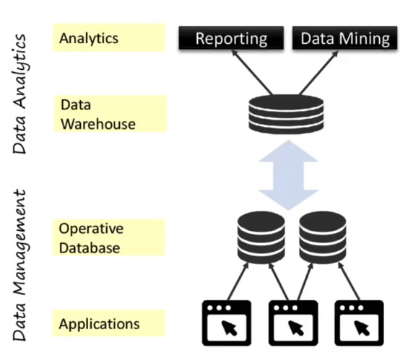
\includegraphics[width=.7\textwidth]{TypicalDataArchitecture.PNG}
    \caption{Typical data architecture.}
    \label{fig_TypicalDataArchitecture}
  \end{figure}

  \begin{proposition}{Typical Data Architecture}
    Organisation tend to have two main data stores
    \begin{enumerate}
      \item A \textit{Data Warehouse} which contains copies of historic data. Data analysis is performed on this data as it is not critical to the operation of the organisation. \textit{Data Warehouses} usually  allow data analysts read-only access.
      \item Several \textit{Operative Databases} which the organisation's core products use and rely on. Data analysis should not be performed on this databases directly as it could interfere with customers (or worse, break the company's products).
    \end{enumerate}
    See \texttt{Figure \ref{fig_TypicalDataArchitecture}} for an illustration.
  \end{proposition}

  \begin{definition}{Datalake}
    TODO
  \end{definition}

\subsection{Storage Technologies}

  \begin{definition}{BLOB Storage}
    A \textit{Binary Large Object} (BLOB) storage is typically used for large, unstructured files (e.g. images \& backup files).
    \par Due to being unstructured, \textit{BLOB} files are not quick to query and are best used just as a record of the data.
    \par \textit{BLOB} files are generally accessed using a REST-API or an SDK, they are not mountable as a disk and drivers need to be build into applications in order for the app to acess the \textit{BLOB Storage}. \textit{Spark} is a tool used by many datalakes for \textit{BLOB} storage.
    \par Data storage providers typically offer two tiers of \textit{BLOB} storage
    \begin{enumerate}
      \item \textit{Hot Access} - Data is accessed frequently.
      \item \textit{Cold Access} - Data is not accessed very often. (Cheaper, but less availability).
    \end{enumerate}
  \end{definition}

  \begin{definition}{Disk Storage}
    \textit{Disk Storage}\footnote{AKA \textit{Block Storage}.} are an alternative form of storage, but are essentially a facade for \textit{BLOB-backed storage} and tend to be up to 1TB in size.
    \par \textit{Disk Storage} can be mounted to a virtual machine. Once mounted and formatted, the file is accessible like any other local file, but with greater throughput than standard-file-storage (60/sec per blob)\footnote{Throughput is lower than \textit{BLOB Storage}.}
    \par \textit{Disk Storage} is ideal when you want to move applications which you were using locally into cloud storage, and you want the data to be decoupled from the virtual machine\footnote{As, otherwise, if the machine was to die then you would loose your data too!}. But, only one person can access a \textit{Disk Storage} at a time.
  \end{definition}

  \begin{definition}{File Storage}
    \textit{File Storage}\footnote{AKA \textit{Network Attached Storage} (NAS).} uses bytes across a network and a using a protocol (e.g SMB), this creates the illusion of the data being a local files. This means several instances of an application can access the data at the same time.
    \par \textit{File Storage} can be upto 5TB each and has a maximum throughput of 60MB/sec across a share\footnote{Slower than BLOB \& Disk}. Throughput is better in Local-Area networks.
    \par \textit{File Storage} is backed by \textit{BLOB Storage} and thus is just as durable.
    \par Capabilities such as concurrency and file locking can be introduced into \textit{File Storage}, availability depends on the protocol being used.
  \end{definition}

\subsection{Databases}

  \begin{remark}{Database Classification}
    There are two features typically used to classify databases
    \begin{enumerate}
      \item The model they use to store data.
      \item Their ``Consistency/Availability'' trade-off.
    \end{enumerate}
  \end{remark}

  \begin{figure}[H]
    \centering
    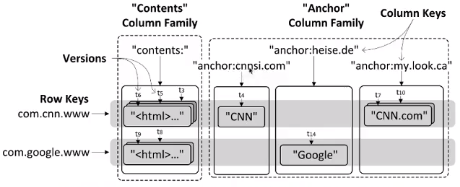
\includegraphics[width=.7\textwidth]{ColumnStores.PNG}
    \caption{Example of data may be structured in a \textit{Colum Store}.}
    \label{fig_ColumnStores}
  \end{figure}

  \begin{definition}{Relational Database}
    TODO
  \end{definition}

  \begin{definition}{Database Models}
    Databases typically use one of the following five models to store \& organise data.
    \begin{enumerate}
      \item \textit{Key-Value Stores} - A dictionary (keys map to values in a deterministic fashion). These databases only support get \& put operations\footnote{There is no support for operations beyond simple CRUD (Create-Read-Update-Delete)}, and all data is stored as a \textit{BLOB}.
      \par \textit{Key-Value Stores} are \textit{schemaless} meaning all assumptions about the structure of the data is implicitly encoded into the application log (and not explicitly defined by a data-definition language).
      \par \textit{Key-Value Stores} are easy to partition, query, have low latency and high throughput.

      \item \textit{Wide-Column Stores} - A distributed, multi-level, sorted map. This means that \textit{Wide Column Stores} have several layers of ``keys'': the first layer, called ``Row Keys'', identify rows which contain a given \textit{key-value pair}; The second layer is known as ``column keys''.\footnote{See \texttt{Figure \ref{fig_ColumnStores}}.} (Columns can be grouped into ``Column Families''. Values in the same column family and same row are stored on the same disk).
      \par \textit{Wide-Column Stores} are space efficient as null values take zero space, and store data in a lexicographic order wrt their keys. Good compression rate allows for efficient querying of row subsets. Versions of each cell can be stored.

      \item \textit{Document Stores} - An implementation of \textit{Key-Value Stores} but each value (known as a ``document'') has to be in a semi-structured format (e.g. JSON). An entire document can be fetched using its unique key. \textit{Document Stores} allow for more complex queries than \textit{Key-Value Stores}, such as: retrieval of parts of documents; aggregation; query-by-example; and, full-text search.

      \item \textit{Graph Databases} - Store data sources in nodes and uses edges to define relationships between data sources. This is really good for complex relationships, but not very scalable as \textit{Graph Partitioning} is NP-Hard.

      \item \textit{Search Engines}\footnote{Not strictly a database} - Essentially an inverted index, with some meta-data and query optimisation. Often will link from a value to the databases which contain that value.
    \end{enumerate}
  \end{definition}

  \begin{remark}{Choosing Database Model}
    When choosing which model of database to use, we are generally trading between the models ability to handle ``size'' and ``complexity''. Generally \textit{Key-Value Stores} are best for the simplest datasets, then \textit{Column Stores}, then \textit{Document Stores} and finally, \textit{Graph Databases} are typically best for handling complex datasets (but do no scale well).
    \par A \textit{Relational Database} is the default model to use for most projects, as they perform well for both size \& complexity up to reasonably large projects.
  \end{remark}

  \begin{theorem}{CAP Theorem}
    The \textit{CAP Theorem}\footnote{Proved by Gilbert and Lynch in 2002.} states that a distributed system or database can guarantee at most two of the following three properties at any one time
    \begin{itemize}
      \item \textit{Consistency} (C) - All users have the same view on the data at all times, with minimal \textit{Latency}.
      \item \textit{Availability} (A) - All users can always read and write to the database.
      \item \textit{Partition-Tolerant} (P) - The system works well across physical network partitions (even if a machine fails or the cluster is split).
    \end{itemize}
  \end{theorem}

  \begin{proposition}{Database Consistency-Availability Trade-Off}
    Databases fulfil one of the following
    \begin{itemize}
      \item \textit{Available \& Partition Tolerant} (AP). (Never a relational database).
      \item \textit{Consistent \& Partition Tolerant} (CP). (Never a relational database).
      \item \textit{Not Partition Tolerant} (CA).
    \end{itemize}
  \end{proposition}

  \begin{definition}{Sharding}
    \textit{Sharding} specifies how data should be partitioning data across several nodes. This is an important technique in data storage as data is often stored in distributed networks.
    \par Here are some popular approachs to \textit{Sharding}
    \begin{itemize}
      \item \textit{Hashing} - Apply a hash function to the data to determine which partition to place it in. Data-pieces which the same hash will be stored on the same machine. \textit{Hashing} creates balanced partitions, but has no data locality.
      \item \textit{Range} - Data-pieces are group according to whether their value falls into a given range. This allows for easier range search and sorting, but is not necessarily balanced.
      \item \textit{Entity-Group} - Explicitly define how to co-locate data. This allows for easy access (equivalent to a single node), but you cannot change the partition after the fact.
    \end{itemize}
    When implementing these approaches we want the partitions to be as balanced as possible, for maximal efficiency.
  \end{definition}

  \begin{definition}{Replication}
    \textit{Replication} is the practice of replicating data so that it is safe should a machine fail. The difficultly in \textit{Replication} is \textit{Sychronisation}.
    \par Here are the two approaches for when to update data
    \begin{itemize}
      \item \textit{Asynchronous} (lazy) - Data is only read on request, this means writing is fast but some replicas may not have been updated (and become stale).
      \item \textit{Synchronous} (eager) - Data is consistent across users, but read-write is slower as the database need to co-ordinate data between users.
    \end{itemize}
    \par Here are the two approaches for where to store data
    \begin{itemize}
      \item \textit{Primary Copy} - A single node accepts write requests and all other nodes just replicate this node. This is quick and easy to keep consistent, but creates a single point of failure.
      \item \textit{Update Anywhere} - Any node can accept write requests, and will then propagate these requests to the rest of the network. This approach is fast to write, but requires co-ordination. This approach is more resilient to hardware failure
    \end{itemize}
  \end{definition}

  \begin{figure}[H]
    \centering
    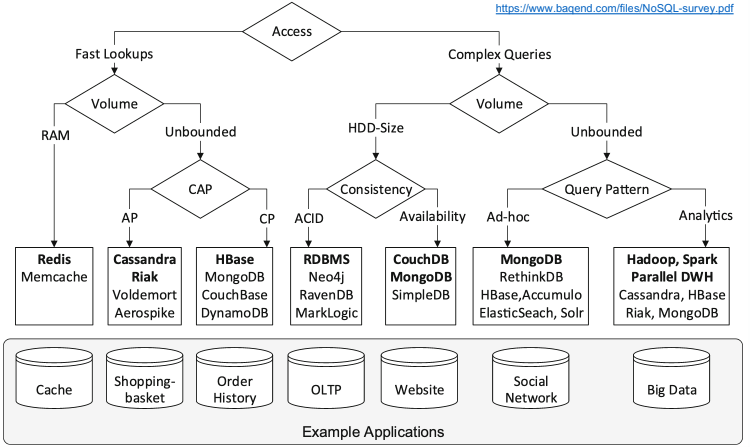
\includegraphics[width=.7\textwidth]{DataStorageFlowChart.PNG}
    \caption{Flow chart to determine which data storage technology to use, given your requirements.}
    \label{fig_DataStorageFlowChart}
  \end{figure}

\subsubsection{Graph Databases}

  \begin{figure}[H]
    \centering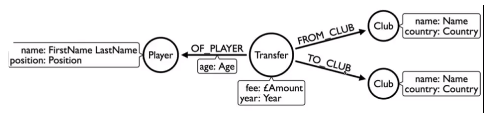
\includegraphics[width=.7\textwidth]{GraphModel.PNG}
    \caption{Example of a graph model for a database storing details about football transfers.}
    \label{fig_graph_model}
  \end{figure}

  \begin{definition}{Graph Model}
    A graph model can be used to represent data dependencies in a database
    \begin{itemize}
      \item \textit{Nodes} are used to represent datafields or tables. Nodes are labelled with the fields which are unique to them.
      \item \textit{Edges} are used to show which nodes depend on each other, often with directionality. Edges are labelled with the fields which are shared (ie connect) between two nodes.
    \end{itemize}
    See \texttt{Figure \ref{sec_storage_and_management}.\ref{fig_graph_model}} for an example.
  \end{definition}

  \begin{figure}[H]
    \centering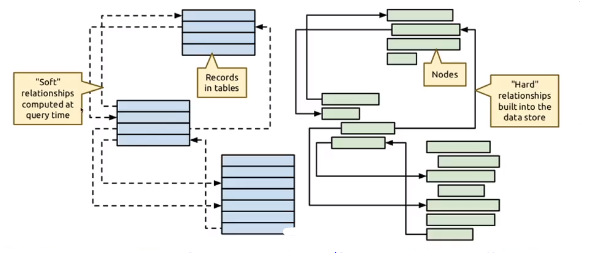
\includegraphics[width=.7\textwidth]{GraphVsRelational.PNG}
    \caption{Comparison of the data-storage architectures for Relation Databases (Left) compared to Graph Databases (Right).}
    \label{fig_graph_vs_relational}
  \end{figure}

  \begin{proposition}{Relational vs Graph Database}
    Here are some comparisons between \textit{Relational} and \textit{Graph Databases}:
    \begin{itemize}
      \item In a \textit{Relational Database} relationships are ``soft'' and only computed at query time.
      \item In a \textit{Graph Database} relationships are ``hard'' as the relationships themselves are stored on the disk.
    \end{itemize}
    See \texttt{Figure \ref{sec_storage_and_management}.\ref{fig_graph_vs_relational}}.
  \end{proposition}

  \begin{proposition}{Neo4J}
    \textit{Neo4J} is a piece of \textit{Graph Database} management software.
    \par Here is an example of a \textit{Neo4J} query\footnote{The equivalent SQL query is \texttt{SELECT * FROM players AS player WHERE player.name = ``Cristiano Ronaldo'';} }
    \begin{quote}
      \texttt{MATCH (player:Player) WHERE player.name = ``Cristiano Ronaldo'' RETURN player;}
    \end{quote}
    In this query \texttt{player} is a variable we create, \texttt{Player} is the type of node that \texttt{player} is and \texttt{name}  is a property of this variable.
    \par We can before logical queries too. The following query returns people who have been a coach \underline{and} a player.
    \begin{quote}
      \texttt{MATCH (n) WHERE n:Player AND n:Coach RETURN n;}
    \end{quote}
  \end{proposition}

  \begin{proposition}{Traversals}
    \textit{Traversals} are a feature which are unique to \textit{Graph Databases}. \textit{Traversals} define what relationship between several nodes to consider, and we can make queries on all these nodes\footnote{Similar to \textit{Joins} in relational databases.}.
    \par The query below fetches all transfers away from Man Utd\footnote{The equivalent SQL query is not as clean \texttt{SELECT from.name FROM transfers AS t JOIN clubs AS clubFrom ON t.from\_club\_id =clubFrom.id WHERE from.name="Manchester United";} }
    \begin{quote}
      \texttt{MATCH (from:Club) <- [:FROM\_CLUB]-(transfer:Transfer)}\\
      \texttt{WHERE from.name="Manchester United"}
    \end{quote}
    \par We can extend this query to be all transfer from Man Utd to Real Madrid\footnote{The SQL for this would require two joins}
    \begin{quote}
      \texttt{MATCH (from:Club) <- [:FROM\_CLUB]-(transfer:Transfer)-[:TO\_CLUB]->(to:Club)}\\
      \texttt{WHERE from.name="Manchester United"}
    \end{quote}
    This query nicely shows how \texttt{<-[]-} and \texttt{-[]->} define the direction of data flow. We can extend this to find any path, including cycles.
  \end{proposition}

  \begin{proposition}{Length of Relationship}
    \textit{Neo4j} allows for variable length relationships. With \texttt{-[:\_\_*n..]->} notation, where meaning a chain of at least \texttt{n} relationships.
    \par The following statement defines a relationship where a player leaves a club and then after some number of transfers returns to the club.
    \begin{quote}
      \texttt{(c:Club)<-[f:FROM\_CLUB]-(sale:Transfer) -[:NEXT*1..]->(rebuy:Transfer)-[t:TO\_CLUB]->(c)}
    \end{quote}
  \end{proposition}

\section{Transformation \& Integration}\label{sec_transformation_and_integration}

\subsection{Data Wrangling}

  \begin{definition}{Data Wrangling}
    \textit{Data Wrangling} is the process of getting to know your data and getting it into a format which you are comfortable with. This should get you interested in the project.
    \par A big part of \textit{Data Wrangling} is detecting inaccurate or malformed records and then correcting or removing them. (Data cleaning, validation, debugging, transforming, formatting, pre-processing).
    \par \textit{Data Wrangling} is an iterative process, you will often return to after ``evaluating your model'' in order to tweak the data some more.
  \end{definition}

  \begin{remark}{Data Used}
    Some \textit{Data Wrangling} tasks need to be performed on the whole data set (e.g. checking \& validation), but others can be performed with a random, representative subset (e.g. exploring)\footnote{You may want to seek out some outliers, especially when your project is interest in outlier cases.}.
  \end{remark}

  \begin{remark}{Strategies for Data Wrangling}
    Here are some things to consider when \textit{Data Wrangling}
    \begin{itemize}
      \item \textit{Type Screening} - Ensuring data is the type you expect and want.
      \item \textit{Range Check} - Check data is within legal ranges or categories.
      \item \textit{Illegal Values} - Check data takes legal values.
      \item \textit{Multi-Column Validation} - Data in different columns is consistent.
      \item \textit{Check Unique/Distinct Values} - Check that unique values are reasonable. (Not typos).
      \item \textit{Remove Duplicates} - Remove duplicate records.
    \end{itemize}
  \end{remark}

  \begin{remark}{Tools}
    There are several useful tools for \textit{Data Wrangling}, including
    \begin{itemize}
      \item Data Wrangler \url{http://vis.stanford.edu/wrangler/}
      \item Pandas.
      \item Regular Expressions.
    \end{itemize}
  \end{remark}

  \begin{remark}{NoSQL Databases}
    \textit{NoSQL Databases} (e.g. MongoDB, Neo4j) are not as strongly typed as SQL databases.
  \end{remark}

  \begin{remark}{Missing Data}
    Missing data is common and can occur for many reasons
    \begin{itemize}
      \item Data may be sensitive and people choose to withhold.
      \item Data may be deemed irrelevant and skipped.
      \item Data may be censored.
      \item Communication link may fail (battery dies).
      \item Data collection may be aborted (boredom).
      \item Data may be corrupted.
      \item Data may not be known by the respondent.
    \end{itemize}
  \end{remark}

  \begin{remark}{Informative Missing Data}
    Sometimes the fact that data is missing can be very informative. It can indicate that the technique/equipment used to take a reading was changed, potentially due to a change in circumstances (A patient went into/out of intensive case).
    \par Imputing values in this case would loose this information.

  \end{remark}

  \begin{remark}{Dealing with Missing Data}
    Here are some approaches which can be taken to deal with missing data
    \begin{itemize}
      \item Cross reference against validated external information.
      \item Impute values from nearest neighbours.
      \item Impute value from mean/median/mode.
      \item Impute from a model-based calculation.
      \item Perform multiple imputations.
      \item Use a ``Missing Data'' indicator.
    \end{itemize}
  \end{remark}

\subsection{Data Fusion}

  \begin{definition}{Data Fusion}
    \textit{Data Fusion} is the process of taking data from different places it and representing it in a single place\footnote{e.g. Having a robot with multiple sensors, and using the accumulated data to determine the robots actions.}. This should create value my increasing the amount of available data.
  \end{definition}

  \begin{figure}[H]
    \centering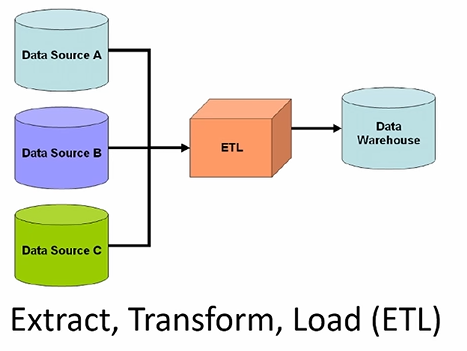
\includegraphics[width=.7\textwidth]{ETL.PNG}
    \caption{Example of an Extract Tranform Load approach to \textit{Data Fusion}.}
    \label{fig_ETL}
  \end{figure}

  \begin{proposition}{Extract. Transform, Load (ETL)}
    \textit{Extract. Transform, Load} (ETL) is an approach to \textit{Data Fusion} where all the data sources are centralised.
    \par See \texttt{Figure \ref{fig_ETL}} from an example.
  \end{proposition}

  \begin{figure}[H]
    \centering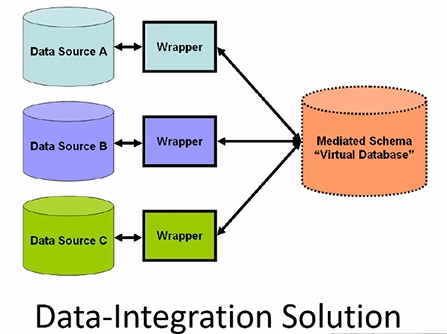
\includegraphics[width=.7\textwidth]{DataIntegration.PNG}
    \caption{Example of an Data-Integration approach to \textit{Data Fusion}.}
    \label{fig_data_integration}
  \end{figure}

  \begin{proposition}{Data-Integration Solution}
    \textit{Data-Integration Solution} is an approach to \textit{Data Fusion} where ``wrappers'' are created for each data source, allowing each to be read using the same schema.
    \par See \texttt{Figure \ref{fig_data_integration}} from an example.
  \end{proposition}

  \begin{definition}{Data Heterogeneity}
    \textit{Data Heterogeneity} is the property that datasets can vary. Data can be different in may ways, including
    \begin{itemize}
      \item Temporally.
      \item Spatially.
      \item Encoding used.
      \item Collection method.
      \item Units of measurement.
      \item License.
      \item Whether missing values have been imputed.
    \end{itemize}
  \end{definition}

  \begin{remark}{Other Issues for Data Fusion}
    Here are some issues which may affect the robustness of some \textit{Data Fusion} methods
    \begin{itemize}
      \item Bad Data - Even if a small part of the data is corrupted then the all the data is compromised.
      \item Lack of Storage - \textit{Data Fusion} methods which centralise all the data will need large disk capacity.
      \item Original Data Sources - If you are interacting with third-party data sources there is a greater risk it will change/be taken down.\footnote{Documentation for data sources will often help alleviate this.}
    \end{itemize}
  \end{remark}

  \begin{definition}{Object Relational Mapping}
    \textit{Object Relational Mapping}\footnote{Examples - Django, MonoEngine, Hibernate.} is an approach to aggregating data from multiple data sources into ``virtual databases'' by creating an interface between the user and the data sources. This makes incompatible data sources ``appear'' compatible. This interface is designed to be flexible and easy to use.
    \par This should speed-up development and allow for migration to be handled automatically. But, gives the user less control (often making complex queries very difficult) and has slower execution speed than directly interacting with the data sources.
    \par \textit{Object Relational Mappings} are often optimised for certain common queries.
  \end{definition}

\section{Exploration \& Visualisation}\label{sec_exploration_and_visualisation}

  \begin{remark}{Common Questions about Data}
    Here are three common early questions we may have about some data
    \begin{enumerate}
      \item What is the average of the sample?
      \item What is the spread of the sample?
      \item What is the effect of outliers?
    \end{enumerate}
  \end{remark}

  \begin{definition}{Inferential Statistics}
    \textit{Inferential Statistics}\footnote{AKA Inductive Statistics} summarise a \underline{sample} and are based on probability theory.
  \end{definition}

  \begin{definition}{Descriptive Statistics}
    \textit{Descriptive Statistics} describe or summarise a \underline{dataset}. \textit{Descriptive Statistics} are useful for assessing data quality, developing models and improving our general understanding about a dataset.
  \end{definition}

  \begin{definition}{Variables}
    There are several classes of variable
    \begin{itemize}
      \item \textit{Qualitiative Variables} - Categorical or discrete data. (inc. nominal, ordinal)
      \item \textit{Quantitative Variables} - Continuous data. (inc. intervals \& ratios)
    \end{itemize}
  \end{definition}

  \begin{definition}{Univariate Measures}
    \textit{Univariate Measures} are measures which describe only one characteristic of a sample/dataset. There are several classes of \textit{Univariate Measures}
    \begin{itemize}
      \item \textit{Central Tendency} (e.g. mean, median, mode).
      \item \textit{Variabiltiy} (e.g. variance,quartiles,max,min,skew). See \texttt{Definition \ref{sec_exploration_and_visualisation}.\ref{def_measures_of_variability}}
      \item \textit{Graphical formats} (e.g histograms).
    \end{itemize}
  \end{definition}

  \begin{remark}{Deciding which ``Central Tendency'' measure to use}
    Plotting a \textit{Histogram} of the data will help decide between using mean, median or mode due to being able to observe the distribution and existence of outliers.
  \end{remark}

  \begin{proposition}{Measures of Variability}\label{def_measures_of_variability}
    Here are some measures of variability in a data set
    \begin{itemize}
      \item Range $\max-\min$.
      \item Variance $\var(X):=\frac1n\sum(X_i-\mu)^2$.
      \item Unbiased variance $\var(X)=\frac1{n-1}\sum(X_i-\mu)^2$.\footnote{Accounts for how sample mean varies $\bar{X}$ from true mean $\mu$}
      \item Standard deviation $\sigma=\sqrt{\var(X)}$.
      \item Quantiles - Values at which $\frac14,\frac12,\frac34$ lies beneath.
      \item Percentiles - Values at which $N\%$ of the data lies beneath.
    \end{itemize}
  \end{proposition}

  \begin{definition}{Raw Moments}
    Let $X$ be a random variable. The \textit{$n^{th}$ Raw Moment} of $X$ is defined as
    \[ \expect[X^n] \]
    This means that the first moment is the expected value and the variance can be derived from the first two moments.
  \end{definition}

  \begin{definition}{Central Moment $\mu_n$}
    Let $X$ be a random variable. The \textit{$n^{th}$ Central Moment} of $X$ is defined as
    \[ \mu_n:=\expect[(X-\expect[X])^2] \]
    The zeroth central moment is 1; first central moment is the expected value; the second central moment is the variable.\footnote{The third and fourth central moments are used to define skewness and kurtosis, respectively.}
  \end{definition}

  \begin{definition}{Standardised Moments $\bar{\mu_n}$}
    The $n^{th}$\textit{Standardised Moment} is the ratio of the $n^th$ centralised moment and the standard deviation to the power of $n$
    \[ \bar{\mu_n}:=\frac{\mu_n}{\sigma^n}=\frac{\expect[(X-\mu)^n]}{(\sqrt{\expect[(X-\mu)^2]})^n} \]
    \textit{Standarised Moments} differ in proeprties other than variability, allowing for comparison of shape of distributions.
  \end{definition}

  \begin{remark}{Cumulants}
    \textit{Cumulants} are another alternative to moments but they seem niche so I cba to define them.
  \end{remark}

  \begin{definition}{Skewness}
    \textit{Skewness} is a measure of distribution shape, describing how lopsided a distribution is.
    \[ \text{Skew}[X]:=\expect\left[\left(\frac{X-\mu}{\sigma}\right)^3\right]=\frac{\mu_3}{\sigma^3} \]
    $\text{Skew}[X]<0$ means the distribution has more values to the right, and $\text{Skew}[X]>0$ it has more values to the left.
  \end{definition}

  \begin{definition}{Kurtosis}
    \textit{Kurtosis} measures the heaviness of the tail of a distribution, compared to a normal distribution with the same variance.
    \[ \text{Kurt}[X]=\expect\left[\left(\frac{X-\mu}{\sigma}\right)^4\right]=\frac{\mu_4}{\sigma^4} \]
    Since the \textit{Kurtosis} of a normal is $3\sigma^4$, we define \textit{Excess Kurtosis} as $\text{Kurt}[X]-3$.
  \end{definition}

\subsection{Data Transformation}

  \begin{definition}{Variance Stabilising Transforms}
    \textit{Variance Stabilising Transforms} are a set of transforms which ensure the variance of each observation is approximately the same. This can be difficult in some cases as the variance may not be constant, but it is related to the mean\footnote{i.e. For a poisson distribution $\var(X)=\expect[X]$.}
    \par A \textit{Box-Cox Transformation} is one such transform.
  \end{definition}

  \begin{definition}{Decorrelation}
    \textit{Decorrelation} is the practice of removing correlation between different variables. This emphasises the differences between variables, allowing for more data to be extracted.
    \par \textit{Principle Component Analsysis} is a \textit{Decorrelation} method.
  \end{definition}

  \begin{proposition}{Decorrelation - Maths}
    \textit{Decorrelation} transforms data st it has a diagonal \textit{Convariance Matrix} $\Sigma=X^TX$. This is done by finding the eigenvaluse of
    \[ \Sigma\Phi=\Phi\Lambda \]
    where $\Lambda$ is a diagonal matrix of eigenvalues and the columns of $\Phi$ are the eigenvectors of the covariance matrix (i.e. $\Phi$ diagonalises $\Sigma$). Equivalently
    \[ \Phi^T\Sigma\Phi=\Lambda \]
    We can decorrelate a single vector $x_i$ (at test time) by calculating
    \[ \hat{x}_i:=\Phi^Tx_i \]
  \end{proposition}

  \begin{definition}{Whitening Data}
    \textit{Whitening Data} is the practice of transforming data such that all variables have the same mean and variance. This makes the data more comparable.
  \end{definition}

  \begin{proposition}{Whitening Data - Maths}
    When \textit{Whitening Data} we are ensuring the eigenvalues in $\Lambda$ are all the same. As eigenvalues determine the length of eigenvectors, ensuring all eigenvalues are the same makes the covariance matrix $\Sigma$ spherical (rather than elliptical).
  \end{proposition}

  \begin{remark}{When to Whiten Data}
    There are some scenarios when it is not good to \textit{Whiten Data}, including
    \begin{itemize}
      \item When the scale of data is important to your inference problem. In this case, eigenvalues could be a useful set of features for inference.
      \item The covariance matrix may be computationally intractable. And, eigenvalues decomposition takes $O(n^3)$ time.
      \item In machines learning you need to use the exact same transformation on training and testing data. These transformations are determined using the training data.
    \end{itemize}
  \end{remark}

\subsection{Density Estimation}

  \begin{definition}{Density Estimation}
    \textit{Density Estimation} is the process of computing the probability distribution which underlies the data. There are two main approaches\footnote{There are also \textit{Semi-Parametric Methods} such as the Dirichlet Process Mixture Model.}
    \begin{enumerate}
      \item \textit{Parametric Approach} - Assume the histogram of the data follows some common-simple distribution\footnote{Often a gaussian}, this means we only need to estimate the parameters of this distribution (mean, variance). This can be extended using \textit{Gaussian Mixture Models}\footnote{A collection of Gaussians each with a different weighting, fitted using the \textit{Expectation-Maximisation Algorithm}.}
      \par A limitation of this is that we are encoding our assumptions into the model, which may not be sound.
      \item \textit{Non-Parametric Approach} - Use the histogram of the data as the distribution. This does not require prior knowledge and inference is easy, but is computationally expensive. This can be extended using \textit{Kernel Density Estimation}.
    \end{enumerate}
  \end{definition}

  \begin{definition}{Kernel Density Estimation}
    \textit{Kernel Density Estimation} uses the following formula to estimate the density $\hat{f}_h(x)$ from the data $\{x_1,\dots,x_n\}$
    \[ \hat{f}_h(x)=\frac1n\sum_{i=1}^nK_h(x-x_i)=\frac1{nh}\sum_{i=1}^nK\left(\frac{x-x_i}h\right) \]
    where $K$ is a smoothing kernel.
  \end{definition}

\subsection{Multi-Variate Analysis}

  \begin{definition}{Multivariate Analysis}
    \textit{Multivariate Analysis} is performed on samples which consist of multiple variables. \textit{Descriptive Statistics} are often used to describe the relationship between pairs of variables (e.g. Cross-tabulations, contingency tables \& graphical representations)
  \end{definition}

  \begin{figure}[H]
    \centering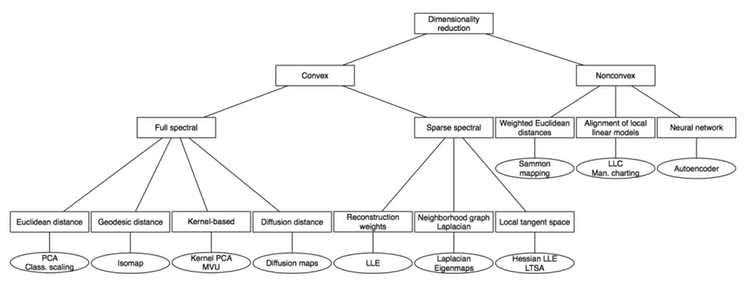
\includegraphics[width=.7\textwidth]{NonLinearDimensionalityReductionTaxonomy.PNG}
    \caption{Taxonomy of methods for non-linear dimensionality reduction.}
    \label{fig_non_linear_dimensionality_reduction_taxonomy}
  \end{figure}

  \begin{definition}{Dimensionality Reduction}
    \textit{Dimensionality Reduction} is the process of reducing the number of variables in each sample, by summarising them.\footnote{Reducing to 2 or 3 dimensions is popular as it is easy to visualise.} We generally choose to do this due to computational limitations.
    \par The two approaches are \textit{Linear Dimensionality Reduction} and \textit{Non-Linear Dimensionality Reduction} (See \texttt{Figure \ref{fig_non_linear_dimensionality_reduction_taxonomy}}).
  \end{definition}

  \begin{definition}{Principle Component Analysis}
    \textit{Principle Component Analysis} (PCA) is a \textit{Linear Dimensionality Reduction} which aims to keep as much variance as possible. Here is the general process to follow
    \begin{enumerate}
      \item Standardise the data.
      \item Obtain the eigenvectors and eigenvalues from the covariance matrix.
      \item Sort the eigenvalues in descending order and choose the $k$\footnote{With $k\ll n$ where $n$ is the number of dimensions in each sample.} eigenvectors which correspond to the largest eigenvalues.
      \item Construct the projection matrix $R\in\reals^{k\times m}$ from these eigenvectors.
      \item Transform the original dataset $X\in\reals^{m\times n}$ using $R$ to obtain $P\in\reals^{m\times k}$.
      \[ P=XR \]
    \end{enumerate}
  \end{definition}

  \begin{definition}{Random Projections}
    \textit{Random Projections} is a simplified version of \textit{Principle Component Analysis} which does not prioritise maximising variability. In the below equation $R$ is chosen at random, we just hope it is good.\footnote{There are extensions we aim to make this more likely.}
    \[ P=XR\]
    where $X\in\reals^{m\times n}$ is data matrix, $R\in\reals^{k\times m}$ is the projection matrix and $P\in\reals^{m\times k}$ is the resulting lower-dimensional representation.
  \end{definition}

  \begin{definition}{Gaussian Random Projections}\label{def_gaussian_random_projections}
    \textit{Gaussian Random Projections} is an extension of \textit{Random Projections} which places restrictions on how $R$ is chosen.
    \begin{enumerate}
      \item First row is a random unit vector, chosen uniformly at random.
      \item Second row is a random unit vector chosen from the space which is orthogonal to the first row.
      \item Third row is a random unit vector chosen from the space which is orthogonal to the first two rows.
      \item etc.
    \end{enumerate}
    This method means that $R$ has \textit{Spherical Symmetry, orthogonality} and \textit{Normality}.
  \end{definition}

  \begin{theorem}{Johnson-Lindenstrauss Lemma}
    Given $\varepsilon\in(0,1)$ a set $X$ of $m$ points in $\reals^n$ and a number $k>\frac8{\varepsilon^2}\ln(m)$, there is a linear map $f:\reals^n\to\reals^k$ st for all $\mathbf{u},\mathbf{v}\in X$
    \[ (1-\varepsilon)\|\mathbf{u}-\mathbf{v}\|^2\leq\|f(\mathbf{u})-f(\mathbf{v})\|^2\leq(1+\varepsilon)\|\mathbf{u}-\mathbf{v}\|^2 \]
    This means generating random projections as described in \texttt{Definition \ref{sec_exploration_and_visualisation}.\ref{def_gaussian_random_projections}} (as they are orthogonal projections) will, in general, reduce the average distance between points.
  \end{theorem}

  \begin{remark}{Database Friendly Random Projections}
    Choosing the elements of our projection matrix $R$ as below is database friendly
    \[ R_{i,j}=\sqrt3\cdot\begin{cases}1&\text{with prob }1/6\\0&\text{with prob }2/3\\-1&\text{with prob }1/6\end{cases} \]
    This is database friendly as elements ar $\{1,0,-1\}$, making the sampling process very simple (easy for a computer).
  \end{remark}

  \begin{definition}{$t$-Distributed Stochastic Neighbour Embedding ($t$-SNE)}
    \textit{$t$-Distributed Stochastic Neighbour Embedding} ($t$-SNE) is a \textit{Non-Linear Dimensionality Reduction} method which tries to capture the relationship between samples and their neighbours (in the high-dimensional space), and then aims to keep these relationships the same in the lower-dimensional space (ie the closest neighbours of each sample are the same before and after transformation).
    \par This is done by modelling the distribution of pairwise similarities as a \textit{Student $t$-Distribution}. Let $P_i$ be the distributions of pairwise similarities for input objects and $Q_i$ for the distribution after the transformation. The problem is now to minimise the distance between the two, this is done by minimising the cost function\footnote{Generally using stochastic gradient descent.}
    \[ C=\sum_iKL(P_i,Q_i)=\sum_i\sum_jp_{j|i}\ln(p_{j|i}-q_{j|i}) \]
  \end{definition}

  \begin{remark}{Using $t$-SNE}
    \textit{$t$-SNE} is best used after a PCA step, it does not perform well as a pre-processing step. This is due to \textit{$t$-SNE} focusing on pairwise relationships (which is local) and may not do well on the global scope.
    \par Each time \textit{$t$-SNE} is run a different visualisation may occur.
  \end{remark}

\section{Data Science in Production}\label{sec_production}

\subsection{Failure is the Rule}

  \begin{remark}{Failure is the Rule}
    ~90\% of data-science projects fail due to the complexity of the production pipeline for data-science.
    \par A common approach is to ``Fail often and Fail cheaply.''
  \end{remark}

  \begin{remark}{Stages of Production}
    There are the typical stages when applying data-science in production
    \begin{enumerate}
      \item \textit{Planning} - Identify the problem and justifying the need for data-science to be used. If this is successful then you need to plan a strategy, determine a budget, hire staff and outline goals (SMART goals).
      \item \textit{Proof-of-Concept}\footnote{AKA ``Lighthouse Projects'' as they shed light on projects.} - Test approaches on a sample of the data. Explore the available data. Build and verify a model.
      \item \textit{Production} - Set up regular flows of data. Check there is no unreasonable bias in your model. Ensure the correct security and governance\footnote{Regular checks of the models performance and ``alerts'' when odds results occur.} procedures are in place. Pay attention to when new trends are arise which your model needs to be retrained for\footnote{Ideally the model would be continuously learning.}. Account for label drifting\footnote{The labels in the data may change their meaning over time.}.
    \end{enumerate}
  \end{remark}

  \begin{proposition}{Components of the ``Proof-of-Concept'' Step}
    A \textit{Proof-of-Concept} can be broken down into the following steps
    \begin{itemize}
      \item Data Management:
      \begin{itemize}
        \item Data collection.
        \item Data pre-processing.
        \item Data augmentation.
        \item Data analysis.
      \end{itemize}
      \item Model Learning:
      \begin{itemize}
        \item Model selection.\footnote{In a business setting you often need to model to be interpretable and some-what agree with preconceptions of your stakeholders.}
        \item Training.
        \item Hyper-parameter selection.
      \end{itemize}
      \item Model Verification:
      \begin{itemize}
        \item Requirement encoding.
        \item Formal verification.
        \item Test-based verification.
      \end{itemize}
    \end{itemize}
  \end{proposition}

  \begin{proposition}{Components of the Production Step}
    The \textit{Production Step} can be broken down into the following steps
    \begin{itemize}
      \item Model deployment
      \begin{itemize}
        \item Integration.
        \item Monitoring.
        \item Updating
      \end{itemize}
      \item Cross-cutting aspects
      \begin{itemize}
        \item Ethics.
        \item End users' trust.
        \item Security.
      \end{itemize}
    \end{itemize}
  \end{proposition}

\subsection{Engineering Guarantees for Data Science}

  \begin{figure}[H]
    \centering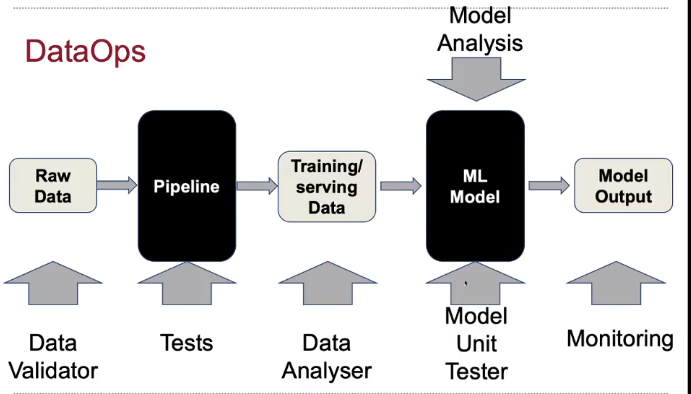
\includegraphics[width=.7\textwidth]{DataOps.PNG}
    \caption{Data Operations pipline}
    \label{fig_data_ops}
  \end{figure}

  \begin{proposition}{Data Validator}
    A Data Validator should ensure that the data in specific fields is of the type we expect and within expected ranges/formats. This is pretty straight-forward for structured and semi-structured data, for unstructured data (e.g images and text) less validation is possible and you may need to abstract the data before validation.
  \end{proposition}

  \begin{proposition}{Data Analyser}
    A Data Analyser should perform basic statistical procedures to check for bias, distribution skew, clusters etc.. In general, you need to be checking these features constantly in both production and deployment.
  \end{proposition}

  \begin{proposition}{Model Unit Tester}
    A Model Unit Tester looks for errors in the training code using synthetic data. Much of this is similar to standard software testing.
    \par They may also need to perform tests to fulfil regulatory/legal requirements (i.e. the model is explainable).
  \end{proposition}

  \begin{proposition}{Tests on Features}
    Here are some tests which can be performed on a model (other than just visual inspection)
    \begin{itemize}
      \item \textit{Score Decomposition} - (Not recommended these days due to non-linearity).
      \item \textit{Ablation Testing} - Remove features one at a time, retrain and observe the difference.\footnote{Popular but nor recommended due to ``Trigger's Broom Paradox''.}
      \item \textit{Feature Permutation} - Choose a feature and augment its values to something which would never occur IRL and observe how other features compensate. This will demonstrate correlations and thus relevance.
      \item \textit{Top-Bottom Analysis} - Compare distributions of inputs and outputs. This will demonstrate correlations and thus relevance.
    \end{itemize}
  \end{proposition}

  \begin{remark}{Feature Store}
    Some companies make us of a special ``Feature Store'' database where previously used features are stored so that their information is not lost even if they are not used in deployment.
  \end{remark}

  \begin{proposition}{Monitoring}
    We want to monitor the output of the model so when the output falls outside some criteria an alert is triggered and someone can investigate.
    \par Model performance dashboards are often used to help monitoring. These dashboards typically display: model output metrics; data input metrics; and, operational telemetry.
  \end{proposition}

  \begin{proposition}{Dimensions of Testing}
    There are often many different dimensions to consider when testing a model. Almost always you want to test the inputs and outputs, but often you will need to test several models and under different conditions (different cities, markets etc.)
  \end{proposition}

  \begin{proposition}{Comparing Algorithms - Large Dataset}
    Here are some methods for comparing different aspects of several models, when you have access to a large dataset
    \begin{itemize}
      \item \textit{Performance Estimation}
      \begin{itemize}
        \item Two-way holdout method (train-test split).
        \item Confidence interval via normal approximation.
      \end{itemize}
      \item \textit{Model Selection, hyperparameter optimisation and performance estimation}
      \begin{itemize}
        \item Three-way holdout methods (train-validate-test split).
      \end{itemize}
      \item \textit{Model \& algorithm comparison}
      \begin{itemize}
        \item Multiple independent training sets + test sets
        \item McNemar test.
        \item Cochran's Q + McNemar test
      \end{itemize}
    \end{itemize}
  \end{proposition}

  \begin{proposition}{Comparing Algorithms - Small Dataset}
    Here are some methods for comparing different aspects of several models, when you have access to a small dataset
    \begin{itemize}
      \item \textit{Performance Estimation}
      \begin{itemize}
        \item Repeated $k$-fold cross validation without independent test set.
        \item Leave-one-out cross validation without independent test set.
        \item Confidence interval via 0.632(+) bootstrap.
      \end{itemize}
      \item \textit{Model Selection, hyperparameter optimisation and performance estimation}
      \begin{itemize}
        \item Repeated $k$-fold cross validation with independent test set.
        \item Leave-one-out cross validation with independent test set.
      \end{itemize}
      \item \textit{Model \& algorithm comparison}
      \begin{itemize}
        \item Combined 5x2cv F test.
        \item Nested cross-validation.
      \end{itemize}
    \end{itemize}
  \end{proposition}

\section{Sharing \& Privacy}\label{sec_sharing_and_privacy}

\end{document}
